\documentclass[titlepage]{article}
\usepackage[utf8]{inputenc}
\usepackage{listings}

\usepackage{graphicx}
\usepackage[margin=1.0in]{geometry}

%%%%%%%%%%%%%%%%%%%%%%%%%%%%%%%%%%%%%%%%%
% Formal Text-Rich Title Page 
% LaTeX Template
% Version 1.0 (27/12/12)
%
% This template has been downloaded from:
% http://www.LaTeXTemplates.com
%
% Original author:
% Peter Wilson (herries.press@earthlink.net)
%
% License:
% CC BY-NC-SA 3.0 (http://creativecommons.org/licenses/by-nc-sa/3.0/)
% 
% Instructions for using this template:
% This title page compiles as is. If you wish to include this title page in 
% another document, you will need to copy everything before 
% \begin{document} into the preamble of your document. The title page is
% then included using \titleGP within your document.
%
%%%%%%%%%%%%%%%%%%%%%%%%%%%%%%%%%%%%%%%%%

%----------------------------------------------------------------------------------------
%	PACKAGES AND OTHER DOCUMENT CONFIGURATIONS
%----------------------------------------------------------------------------------------

%\documentclass{book}

\newcommand*{\plogo}{\fbox{$\mathcal{UH}$}} % Generic publisher logo

%----------------------------------------------------------------------------------------
%	TITLE PAGE
%----------------------------------------------------------------------------------------

\newcommand*{\titleGP}{\begingroup % Create the command for including the title page in the document
\centering % Center all text
\vspace*{\baselineskip} % White space at the top of the page

\rule{\textwidth}{1.6pt}\vspace*{-\baselineskip}\vspace*{2pt} % Thick horizontal line
\rule{\textwidth}{0.4pt}\\[\baselineskip] % Thin horizontal line

{\LARGE Comparison of Absolute and Relative Pointing Effectiveness \\ using \\[0.3\baselineskip] Leap Motion}\\[0.2\baselineskip] % Title

\rule{\textwidth}{0.4pt}\vspace*{-\baselineskip}\vspace{3.2pt} % Thin horizontal line
\rule{\textwidth}{1.6pt}\\[\baselineskip] % Thick horizontal line

\scshape % Small caps
Interface Technologies \\ % Tagline(s) or further description
%Abstract. \\[\baselineskip] % Tagline(s) or further description
%Abstract.\par % Location and year

\vspace*{2\baselineskip} % Whitespace between location/year and editors

Report Submitted by \\[\baselineskip]
{\Large Afaque Hussain - 014126226 \\ Chris Blythe - 014258961 \\ Farbod Faghihi - 014343410  \\   Maninder Singh - 014343397\\ Payel Bandyopadhyay - 014174692 \\} % Editor list
%{\itshape University of Helsinki \\ Finland\par} % Editor affiliation

\vfill % Whitespace between editor names and publisher logo

%\plogo \\[0.3\baselineskip] % Publisher logo
\begin{figure}[!h]
\centering

\includegraphics[width=1.5in]{Logo_UH}
\end{figure}
%{\scshape 2013} \\[0.3\baselineskip] % Year published
%{\large University of Helsinki, Finland}\par % Publisher

\endgroup}

\begin{document}
\pagenumbering{roman}
%\setcounter{page}{3}
%\maketitle
%\pagestyle {empty}
\titleGP
\clearpage

%\vspace{\fill}
%\begin{document}
%\pagenumbering{alph}
%\begin{abstract}
%This project shows an application that can be used as a research tool to compare the ease of use between absolute pointing and relative pointing using Leap Motion Controller. It captures the quantifiable data in order to assess the effectiveness of different pointing techniques using a Leap Motion Controller. The application consists of four colored circles and four target circles. The user needs to select the colored circles one at a time and drag it to the respective target circles. The same task has to be done for both the pointing modes. For comparing the ease of use, we display the time a single user takes to complete the whole task, in each pointing mode. \\

 
%\end{abstract}
%\vspace{\fill}
%\clearpage

\tableofcontents
\newpage
\pagenumbering{arabic}
\setcounter{page}{1}
\section{Abstract}
This project shows an application that can be used as a research tool to compare the ease of use between absolute pointing and relative pointing using Leap Motion Controller. It captures the quantifiable data in order to assess the effectiveness of different pointing techniques using a Leap Motion Controller. The application consists of four colored circles and four target circles. The user needs to select the colored circles one at a time and drag it to the respective target circles. The same task has to be done for both the pointing modes. For comparing the ease of use, we display the time a single user takes to complete the whole task, in each pointing mode. \\
\newpage
%\setcounter{page}{1}
%\pagenumbering{arabic}
%\begin{document}
%\pagenumbering{roman}
\section{Project URL}
The source code of the project is hosted on GitHub. The project can be cloned using this URL: 

https://github.com/afaquejam/LeapAbsRel.git. 

\section{Introduction}
Pointing is one of the most fundamental way in which users interact with computers. Pointing can be done with different techniques like pointing with help of an eye, pointing with help of a hand etc. In this project, the main focus is pointing with fingers. Figure 1 shows an overview of finger pointing.

\begin{figure}[!h]
\centering

\includegraphics[width=3.5in]{Figure_1}
\caption{An overview of pointing with help of finger.}
\end{figure}

Pointing in a computer is done with various devices like mouse, joystick, trackball, touch-pad. In our project, we develop an application that enables pointing by fingers using a device called as Leap Motion Controller.

Leap Motion Controller is unique from other pointing device in a sense that, using this device as a pointing device, does not require a user to have a direct contact (or touch) with a computer screen. This device allows hand and finger as user inputs to interact with the computer. Figure 2 shows an overview of Leap Motion Controller. Figure 3 shows how a user can interact with the computer with help of Leap Motion Controller.

\begin{figure}[!h]
\centering
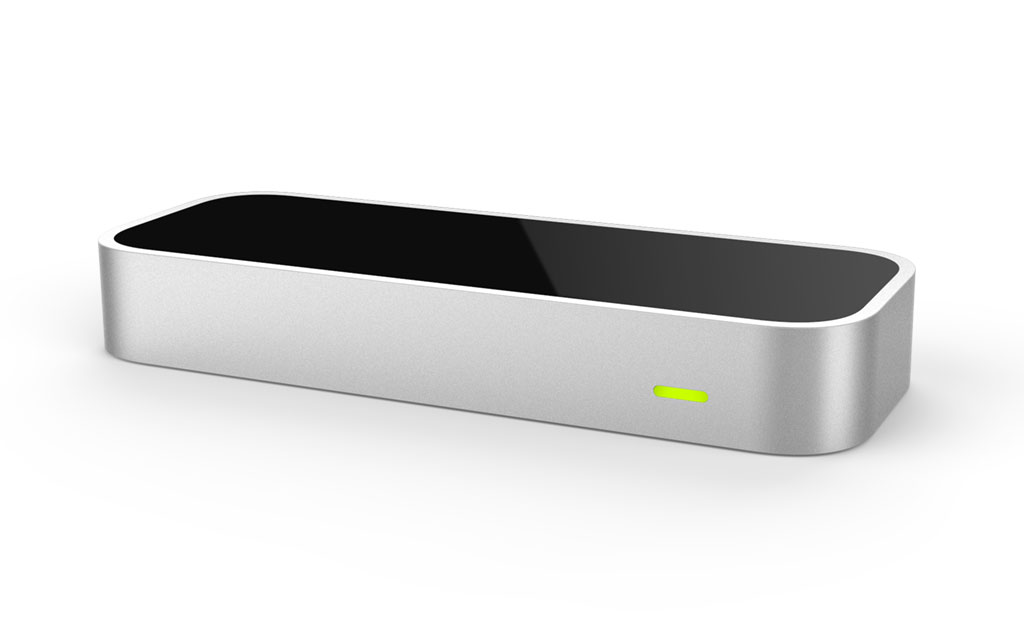
\includegraphics[width=3.5in]{Figure_2}
\caption{A Leap Motion Controller}
\end{figure}

\begin{figure}[!h]
\centering
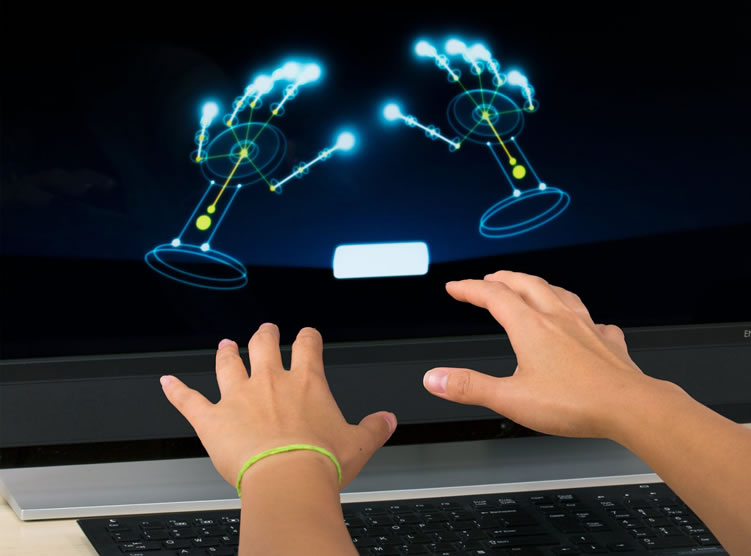
\includegraphics[width=3.5in]{Figure_3}
\caption{A user interacting with a computer using Leap Motion Controller.}
\end{figure}

Pointing are of two types: relative pointing and absolute pointing. Absolute pointing \cite{1} is direct pointing. Direct in this context means that there is a direct relation between the location of the pointing device and the cursor location. Few examples of direct pointing devices are touch screens, light pens and stylus boards. Relative pointing \cite{1} is indirect pointing. Indirect means that the user uses the pointing device to move the cursor from a starting point to an ending point, and there is no direct mapping between the device and the X, Y location on the screen. If the mouse reaches the edge of the mouse pad, the user can pick it up, put it back in the center of the mouse pad, and continue.   

\subsection{Application Description}

{\bf System requirements}:
\begin{itemize}
\item OS - Windows (version 7 or 8)
\item Pointing device - Leap Motion Controller
\item Framework - .NET 3.5 or above
\item Software - Leap Motion Software, Airspace, Unity 4 (Version 4.2.2f1)
\end{itemize}

{\bf Motive of the application}: The application developed in this project shows a comparison of ease of use of absolute pointing and relative pointing using Leap Motion Controller. In this application, a user performs the same task using two different pointing modes. 

{\bf User Interface description}: There are 4 filled balls of same size but different colors. There are 4 target circles of same size but different colors. The colors of the target circles are matched with the respective balls. The size of the target circles are bigger than the filled balls. When a user interacts with computer with help of a mouse, an arrow is shown as a cursor on the interface of the computer. In our project, when a user interacts with our application, a very small purple colored circle is shown as pointing circle (cursor). Whenever a user selects a filled ball, the color of the pointing circle changes. At the top, a timer shows the time to complete a single task.

{\bf Using the application}: The task that a user performs in two different pointing modes is to drag balls (filled with colors) to their respective target circles. The main menu of the application  provides a user (using this application) to choose between relative pointing mode and absolute pointing mode. For user feasibility, the application also provides an option for choosing between space bar grab mode and thumb grab mode. Space bar grab mode means, that the user can drag the filled balls towards the target circles with help of a space bar. Thumb grab mode means that the user can drag the filled balls with help of only thumb. This user feasibility has been introduced because Leap Motion Controller is quite new, hence users might find difficulty in dragging balls within the UI. We had tested our application with 3 users (all of them were new to Leap Motion Controller). All of them found difficulty in dragging the filled balls to their respective target circles, using only the thumb. Hence, we introduced the space bar mode, for user feasibility. After the space bar mode was introduced in the application, we repeated the same experiment with the same 3 users. This time users could use the application in much easier way. We record the time a user takes to complete a task using two pointing modes (absolute pointing and relative pointing).


\section{Background}
The idea of the project lies in showing the difference between relative pointing and absolute pointing. Relative pointing has got no direct relationship between the cursor of the pointing device and the position of the pointing device \cite{2}. On the other hand, absolute pointing there exists a direct relationship between the orientation of the pointing device and the cursor of the computer. These coordinates are gathered from with respect to fixed reference directions (for orientation) or fixed reference locations (for position) \cite{2}. Figure 4 shows the difference between relative pointing and absolute pointing. 

\begin{figure}[!h]
\centering
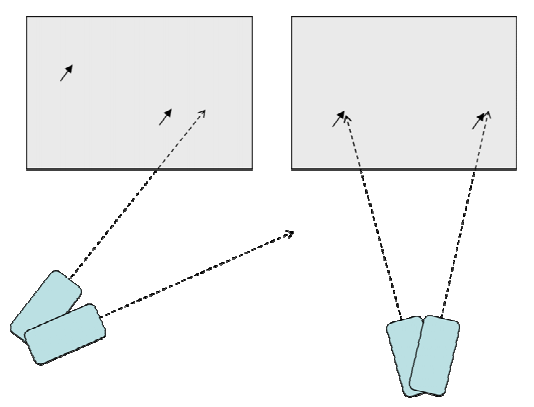
\includegraphics[width=3.5in]{Figure_4}
\caption{Illustrating the difference between relative (left) and absolute (right) pointing \cite{2}.}
\end{figure}

In our project, we demonstrate the difference between absolute pointing and relative pointing with the help of fingers. Vogel and Balakrishnan \cite{3} provide a design which demonstrates freehand pointing and clicking interaction with very large high resolution displays from a distance. The authors discuss about “Clicking and Clutching Without a Button”, which is the key point of our project. The authors have used hand gestures and postures for clicking. They argue that the click or clutch action should be designed in such manner that it minimizes hand movement side effects. This can be tedious due to the interconnectedness of tendons and ligaments in the hand. When a user selects or clicks a button, proper user feedback should be given so that the user is confirmed that the user has performed the task correctly. All of these user feed-backs are taken care of in our application.

\begin{figure}[!h]
\centering
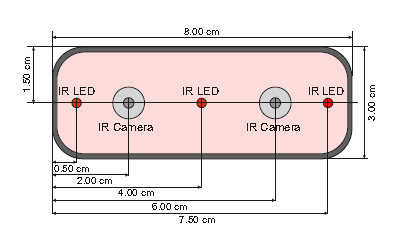
\includegraphics[width=3.5in]{Figure_5}
\caption{A schematic view of Leap Motion Controller \cite{4}.}
\end{figure}

Weichert et al. \cite{4} discuss about a new pointing device called Leap Motion Controller. This device has been used as the base of pointing device in our application. The Leap Motion Controller introduces a new methodology of interaction with the computers. It introduces a new gesture and position tracking system with sub-millimeter accuracy. The authors have shown the accuracy and robustness of the Leap Motion Controller. The controller is available to public and is currently been produced by Leap Motion \cite{5}. This controller calculates position in Cartesian space of predefined objects like finger tips, pen tip, etc. \cite{4}. These positions are in relation to the Leap Motion controller’s center point. The center point of the controller second infrared emitter. Figure 5 shows the schematic view of the Leap Motion Controller. The middle infrared emitter is the center point. It also consists of two infrared cameras. 

\section{Design}
This application allows a user to drag the circles to their respective target circles using two pointing modes (absolute pointing and relative pointing). The time to accomplish the task using both the pointing modes are being recorded. This application can act as a tool to compare between the two pointing modes to see if there are any identifiable differences in how effective each mode is compared to the other using Leap Motion Controller. 

The main concepts of the design of this application is modular design. The key design concepts are:

\begin{itemize}
  \item Separate scripts interacting with each other.
  \item Separation of UI from behaviour implementation.
\end{itemize}

\begin{figure}[!h]
\centering
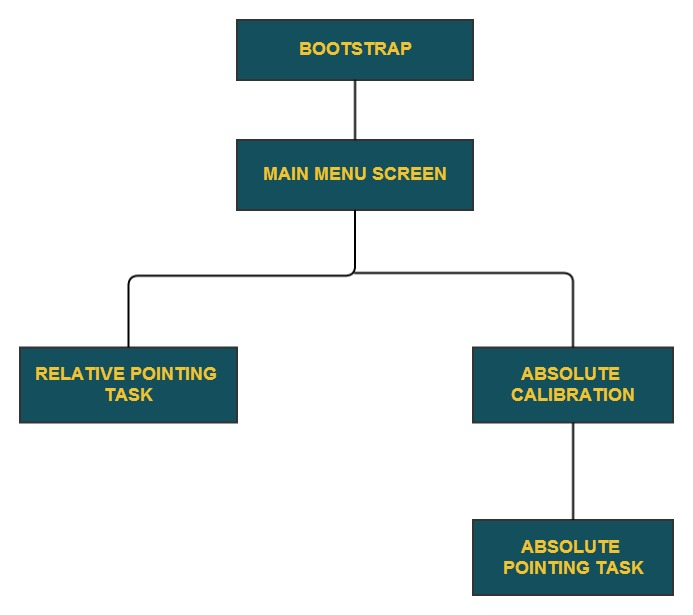
\includegraphics[width=4.5in]{Figure_6}
\caption{A higher level architecture of the application of this project.}
\end{figure}

The scripts responsible for user interface are:

\begin{itemize}
    \item Pointer.cs
    \item Circles.cs
    \item TaskTimer.cs
    \item KeyboardInput.cs
    \item LeapAsMouse.cs
    \item TitleGUI.cs
\end{itemize}

The scripts responsible for implementing the absolute and relative pointing concepts are:

\begin{itemize}
    \item LeapPointing.cs
    \item AppData.cs
    \item AbsoluteCalibration.cs

\end{itemize}

Figure 6 shows an overview of the higher level architecture of the application. The figure shows the main Unity scenes of the application.

The Bootstrap scene consists the following scripts:

\begin{itemize}
    \item AppData.cs
    \item KeyboardInput.cs
    \item LeapPointing.cs
\end{itemize}

KeyboardInput.cs script captures the keyboard input and updates global AppData. It uses the AppData to communicate with other scripts. The LeapPointing.cs script contains the code for both absolute pointing mode and relative pointing mode. This script updates the AppData.cs script with coordinates to communicate with other modules depending on the pointing mode selected in AppData. The AppData.cs script stores all the data that is used across multiple scenes. Figure 7 shows the functionality of the bootstrap scene.

\begin{figure}[!h]
\centering
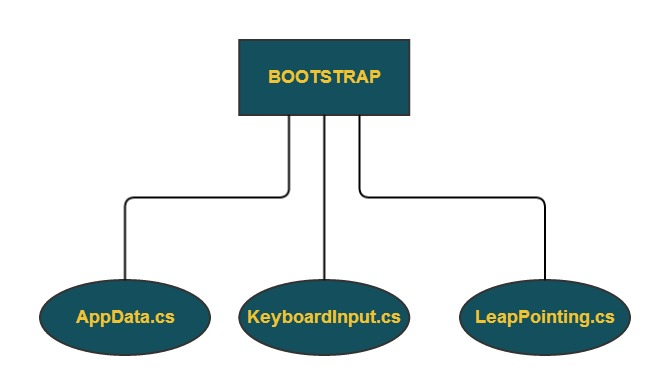
\includegraphics[width=4.5in]{Figure_7}
\caption{A higher level architecture of the application of this project.}
\end{figure}


The Bootstarp.cs script calls the main menu scene. It is to load the persistent DataObject to avoid duplication. The main menu scene consists of TitleGUI.cs script. It consist the user interface of the main menu. Figure 8 shows an overview of the interface of the main menu. This allows the user to choose between the two types of pointing modes. After choosing the required pointing mode, the user moves to the main application task area where the user performs the task of dragging circles.

\begin{figure}[!h]
\centering
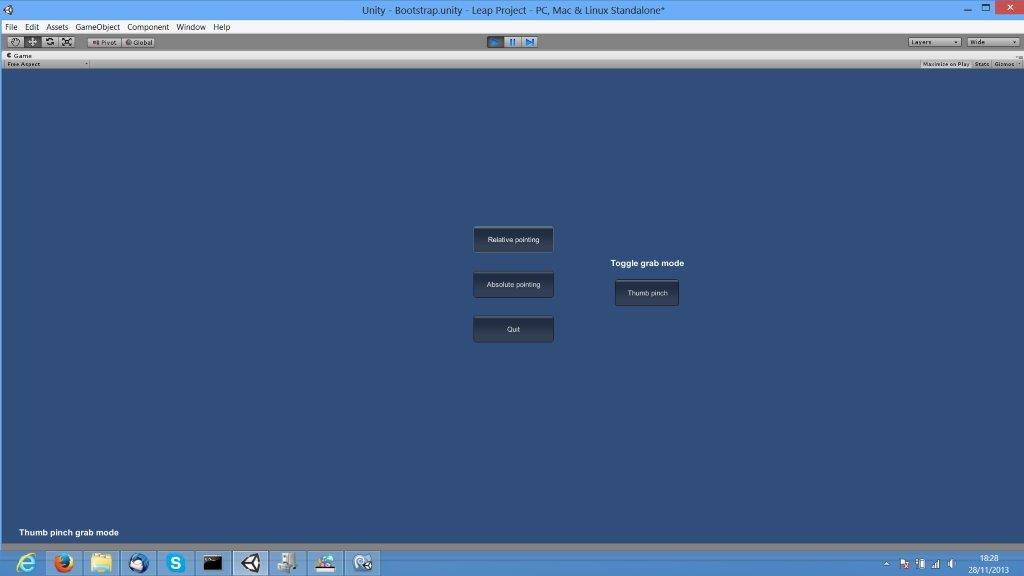
\includegraphics[width=7.0in]{Figure_8}
\caption{A screenshot of the main menu of the application.}
\end{figure}

The relative pointing task scene consists of the following scripts:

\begin{itemize}
    \item Pointer.cs
    \item Circles.cs
    \item TaskTimer.cs
\end{itemize}

Pointer.cs script draws purple colored pointer (which acts as cursor) to the screen coordinates. It updates the coordinates from the AppData.cs script. The Circles.cs script draws 4 circles and 4 target circles on the screen. It also records state of the circles - grabbed or not grabbed. If the user successfully grabs or selects a ball, then it changes the color of the circles. It also redraws the circles if the user cannot successfully drag the ball inside the target circles. The application also changes color when the center of the ball and the target circle matches providing a user feedback. The TaskTimer.cs script displays the time taken for a user to complete the full task of drag and drop of circles to the target circles. It starts recording the time when a user first selects a ball for dragging and ends when the user successfully drops the last ball to the target circle. Figure 9 shows internal flow diagram of relative pointing task scene. 

\begin{figure}[!h]
    \centering
    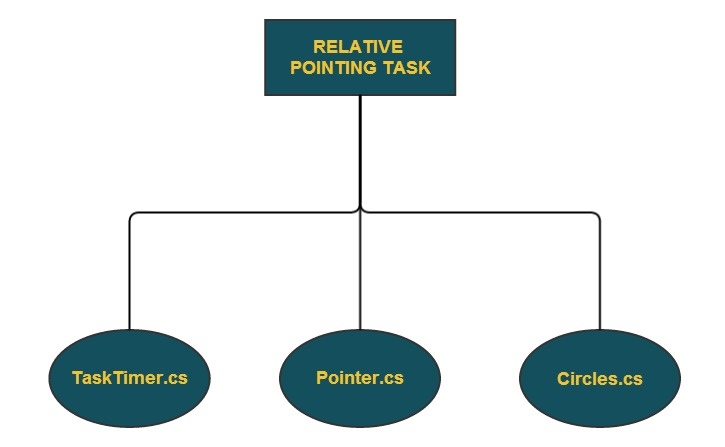
\includegraphics[width=4.5in]{Figure_9}
    \caption{Internal flow diagram of relative pointing task scene.}
\end{figure}
 

The AbsoluteCalibration.cs is the most important script for absolute pointing mode. The absoloute pointing mode uses this scaling ratios in its algorithm. The calibration script calculates the scaling ratios to create a relationship between leap position and screen dimensions. For scaling, it calculates the following data points:

\begin{itemize}
    \item 3 top left of screen
    \item 3 bottom right of the screen

\end{itemize}


The relativabsolute pointing task scene consists of the following scripts:

\begin{itemize}
    \item Pointer.cs
    \item Circles.cs
    \item TaskTimer.cs
    
\end{itemize}

The functionalities of each of the scripts have been explained above.

\section{Development}

The most significant elements of the application are the approaches taken for the relative and absolute pointing algorithms. This section provides a brief explanation of the relevant code contained in the LeapPointing script mentioned in the previous scetion.

\subsection{Relative pointing algorithm}
A zone is defined for the leap motion based on predefined values for width and height above table top. This 'zone' is effectively the space a user will be moving their finger around in above the Leap device. The height of the leap zone is then dynamically calculated based on the dimensions of the Unity window resulting in the Leap zone having the same ratio as the Unity screen as shown in Figure 10.

\begin{figure}[!h]
    \centering
    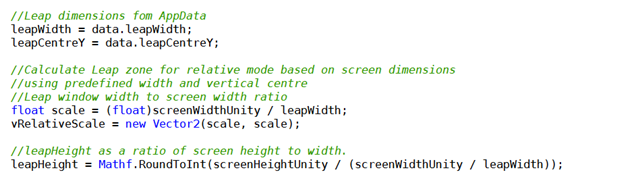
\includegraphics[width=7.0in]{Figure_10}
    \caption{Calculation of Leap zone dimensions.}
\end{figure}

The relative pointing algorithm takes raw data from the Leap in the form of the pre-stabilised position of the frontmost finger. The Leap coordinates (with X axis centred above the Leap device and Y zero located down at the device) are transformed to conform to Unity coordinates (0,0 top left) and adjusted to the dimensions of the previously defined Leap zone as shown in Figure 11.

\begin{figure}[!h]
    \centering
    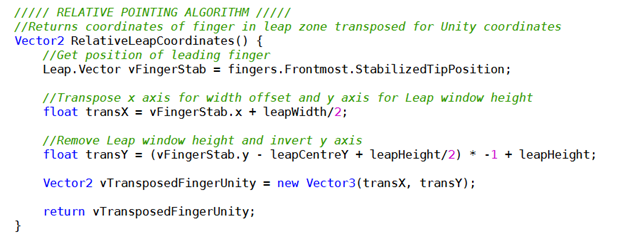
\includegraphics[width=7.0in]{Figure_11}
    \caption{Relative pointing algorithm.}
\end{figure}
 
The StabilizedTipPosition method offered by the Leap has very effective context-sensitive filtering and stabilisation, so no further smoothing is required.

Finally, when the application is in the RelativePointing mode (the relative pointing task screen as shown in Figure 12), the RelativePoint method (as shown in Figure 13) gets the Unity adjusted coordinates from the  relative pointing algorithm and scales them to the screen dimensions using the Leap zone to screen size scaling value calculated in figure 10.

\begin{figure}[!h]
    \centering
    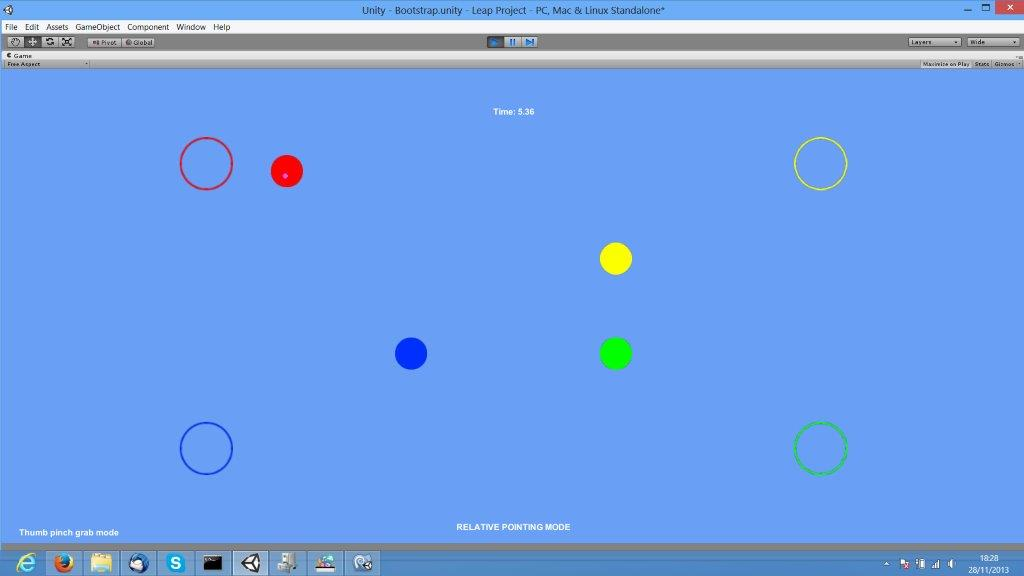
\includegraphics[width=7.0in]{Figure_13}
    \caption{A screenshot of relative pointing task scene of the application.}
\end{figure}


\begin{figure}[!h]
    \centering
    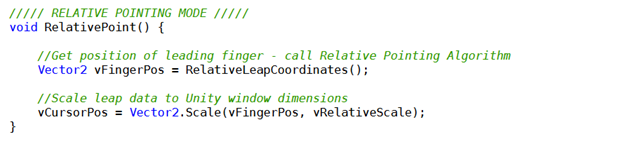
\includegraphics[width=7.0in]{Figure_12}
    \caption{RelativePoint method scaling results from relative pointing algorithm to screen size.}
\end{figure}


\subsection{Absolute Pointing}
The absolute algorithm (as shown in Figure 14) makes use of a Leap feature where the angle of a finger is used to project a line onto a virtual screen which returns a coordinate where the projected line intersects with the virtual screen. Initially the closest finger to the screen is defined. Then a virtual screen that that fingers projected line is intersecting with is identified, and the intersection coordinate is captured in vLeapIntersect. After converting the Leap vector to a Vector2, the coordinates are scaled up from their normalised form to create a virtual screen with coordinates transposed to the Unity system.
 
To create the relationship between the virtual screen and the real screen, reference points (of top left and bottom right), which were defined during calibration, are used. The virtual screen coordinates are scaled to real window coordinates based on the ratio between virtual screen dimensions and the reference points (defining the real screen dimensions).
 
Finally smoothing is applied. This is required as the sensitivity of the Leap device means the pointer jumps around the screen due to natural tremors in the pointing finger.

\begin{figure}[!h]
    \centering
    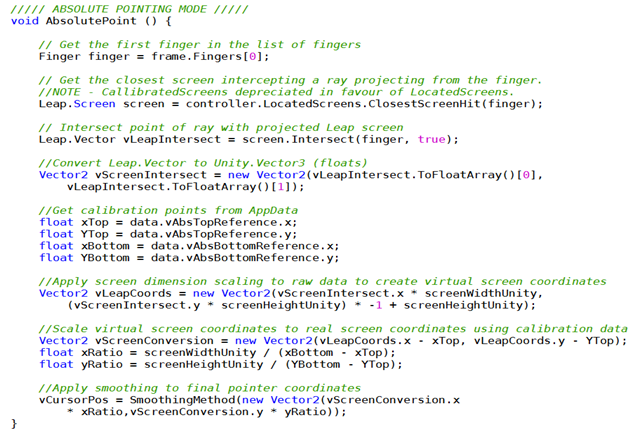
\includegraphics[width=7.0in]{Figure_14}
    \caption{Absolute pointing algorithm.}
\end{figure}

The smoothing algorithm (as shown in Figure 15) employs a Savitzky-Golay algorithm. It applies weighting coefficients to the last 9 frame coordinates giving prominence to the coordinates in the middle of the data set. This effectively fits the data into a polynomial which reduces the impact of noisy coordinates and produces a cosmetic smoothing effect for the pointer on screen.

\begin{figure}[!h]
    \centering
    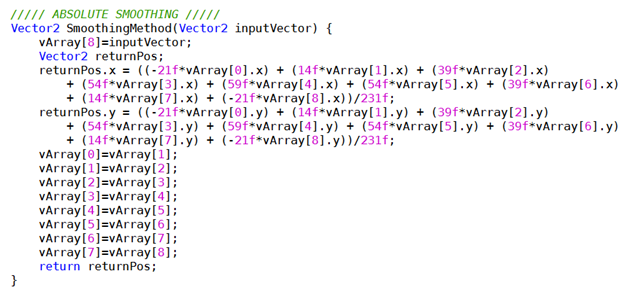
\includegraphics[width=7.0in]{Figure_15}
    \caption{Absolute smoothing algorithm.}
\end{figure}

\section{Discussion}

The application developed in this project shows the comparison of absolute pointing and relative pointing effectiveness with help of Leap motion controller. Figure 16 shows what a user achieves at the end of completing a task in absolute pointing mode. As mentioned earlier, the same task is achieved in relative pointing mode also.
\begin{figure}[!h]
    \centering
    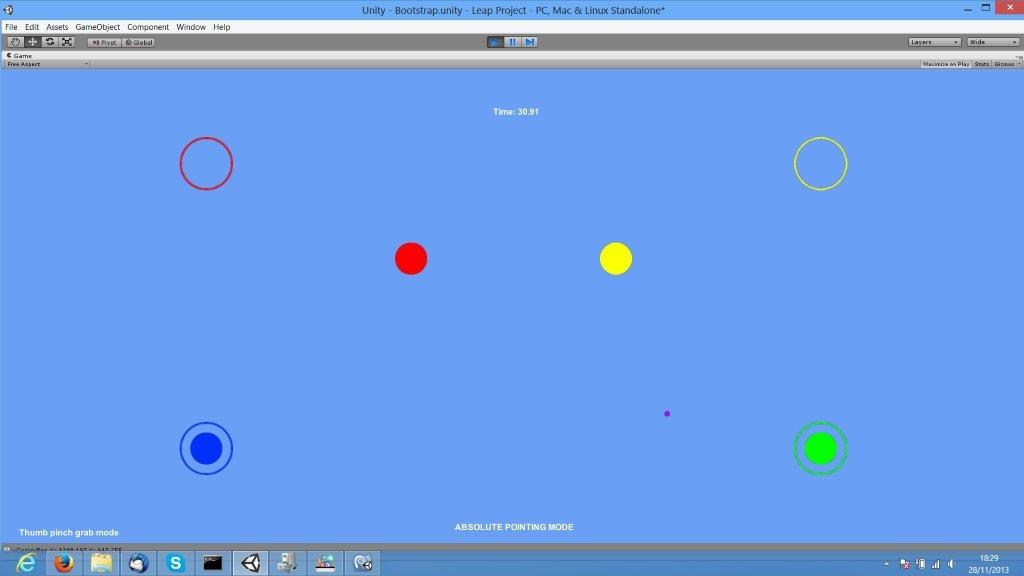
\includegraphics[width=6.0in]{Figure_16}
    \caption{A screenshot of absolute pointing screen that a user achieves after completing the task.}
\end{figure}

While development of this application, number of challenges were faced. The very first challenge we faced was to narrow down to the programming language to be used for developing applications which use Leap Motion. As Leap Motion is still in its infancy, the documentation is not easy to follow, although its getting better. Regarding the development of the application, the challenge was, according to the documentation of Lead SDK, it could be used as a plug-in in a Unity application using Pro version of Unity. Anyways using some tweaks, we got it to interact with a sample unity application using leap motion with a free version too. The next challenged faced was with Unity support for 2D graphics. Unity inherently provides a 3D development environment, hence developing a 2D graphical user interface in Unity was a challenge. Part of the challenge was the poor support Unity provided for 2D graphics, and we had to use the limited GUI functions in Unity to draw everything. The other disappointing aspect of this was to loose a great deal of Unity's power in the form of object configuration and reuse. Although we worked hard to modularise code in the form of multiple interacting scripts, all the graphical elements had to be drawn procedurally from within scripts. Controlling the mouse cursor from within Unity was our next challenge. Initially we expected to use the mouse cursor on screen and control its position using the Leap motion. However it turned out it is difficult to do and research on the web consistently returned the answer that it was not possible (Unity had no explicit way of  controlling the mouse). To solve this we implemented our own 2D texture (the purple spot) to use as an on screen pointer. Later, during a discussion with Imtiaj  (our project tutor), we found out a way of importing user32.dll and using it to access native mouse commands and position. We implemented this type of cursor control on the menu screen and kept the graphical cursor for the pointing task scenes.

The next challenge was getting desired usability for users to be able to complete the tasks. Although working out how to approach relative pointing using the Leap API was pretty straight forward, it was more of a challenge to deal with the absolute pointing. We were able to see some of the mechanisms used through examining other code examples, but it wasn't until Imtiaj (our project tutor) explained the principles of a line projected from a finger intersecting with a virtual screen that we were able to get to grips with it and work out an implementation in Unity. The last challenge in absolute pointing mode was pointer jitter problems. There were issues with pointer stability due to the Leap Motions high sensitivity and humans natural hand tremors. Hence to overcome this problem smoothing algorithm was used. Initially we implemented a gesture using the thumb for picking up (grabbing) the circles to drag them. When the thumb is extended out at an angle from the forefinger the pointer is 'ungrabbed', and when the thumb is drawn in to lie alongside the hand the pointer grabs any circle it is over. Although this mechanism worked well initially two problems later came to light. During early user testing it was discovered that some peoples hands did not work consistently with the gesture detection implementation and sometimes dropped the circles unintentionally. This was considered to be a major problem if task completion was being timed, as an unintentional drop of a circle would negatively skew the test results and not be a true representation of  pointing usability. The second issue was with absolute pointing. If the thumb grab mode worked for an individual, it worked well in the relative pointing task. However when the absolute pointing algorithm was completed, it was discovered that the sensitivity inherent in absolute pointing (i.e. the small angle change required to point from one side of the real screen to the other) resulted in the pointer drifting when the user made the grab action with the thumb. This made it difficult to pick up the circles on occasions, again negatively effecting the time result. To solve these problems, we added another form of grab control, and allow users to toggle between them allowing a choice. The alternative grab turns off the thumb grab mode and allows the left mouse button or the space bar to be pressed to grab the circles. This has proved to be very effective allowing users to choose how they interact with the application as best suits them.
  
Also, some challenges were faced regarding the softwares used in this project. The Leap Motion controller had stopped working twice. It is a bug of the Controller. After un-installing and reinstalling the leap software, the device started working once again. Unity 3d game engine supports only Mac OSX and Microsoft Windows and in order to work with that some of us had to install Windows in their system. Another problem with Unity was that it does not support Java, they provide something close to Java called UnityScript which is referred to as JavaScript by the software. So in order to edit the code we had to learn UnityScript or C#. In short, the development tools provided by the Unity game engine is somehow limited.

Also, the main requirement of the application development was Leap Motion Controller. Given a team size of 5 members, only one controller was available. If one more controller was available then the development process would have been easier and convenient. The availability of the Leap Motion controller was a problem. 


\section{Conclusion}
This project shows an application that compares the ease of use between absolute pointing and relative pointing using Leap Motion Controller. The finger is considered as the mode of pointing. This project integrates Leap Motion controller with Unity. It captures the quantifiable data in order to assess the effectiveness of different pointing techniques using a Leap Motion Controller. 





\bibliography{if.bib}
\bibliographystyle{plain}

\end{document}
